\documentclass[11pt]{article}
\usepackage[margin=1in]{geometry}
\usepackage{amsmath,amssymb,amsthm}
\usepackage{graphicx}
\usepackage{verbatim}
\usepackage{microtype}
\usepackage{listings}
\lstset{basicstyle=\ttfamily\scriptsize,breaklines=true,breakatwhitespace=false,
  keepspaces=true,columns=fullflexible,showstringspaces=false,
  prebreak=\mbox{\tiny$\hookleftarrow$},frame=none,
  literate={$}{{\char36}}1 {\_}{{\char95}}1 {\^}{{\char94}}1}
\renewcommand{\S}{\mathhexbox278}

\newtheorem{theorem}{Theorem}[section]
\newtheorem{proposition}[theorem]{Proposition}
\newtheorem{conjecture}[theorem]{Conjecture}
\theoremstyle{definition}
\newtheorem{definition}[theorem]{Definition}
\theoremstyle{remark}
\newtheorem{remark}[theorem]{Remark}

\newcommand{\Tr}{\operatorname{Tr}}

\title{Transient Structure at Solar Rigidity Interfaces and the\\
Exceptional Point of the Dynamo Wave:\\
\large An Operator-First Study of the Sun}
\author{Jeromie N.\ Beasley}
\date{August 16, 2026}

\begin{document}
\maketitle

\begin{abstract}
We study the sun as the observable panel of a single operator-theoretic
family: non-normal transport operators whose stress concentrates at rigidity
interfaces, previously developed for the four-body shape manifold and its
black-hole horizon analogue. Two computations carry the paper, each stated as
predictions before it was run and graded afterward. (1) A magnetized shear
layer with the magnetic field inclination as the control dial---the geometry
of the 2026 DKIST observation of vortex chains confined to the boundaries of
photospheric magnetic flux concentrations---shows a measured modal quench at
tilt $30^\circ$--$35^\circ$ and, beyond it, a \emph{directional-rigidity curve}, strictly decreasing over the sampled
tilts: maximum transient energy growth falls
$8.8\to2.3$ and the Kreiss constant falls $1.80\to1.08$ as the field tilts
into the shear. The same run yields an unordered finding---the operator's
commutator stress \emph{rises} while its realizable amplification falls:
tension stores stress without releasing it---and one dimensionless number
fixed by the fastest-growing mode, $\lambda/d=13.96$, from which the
published vortex statistics can be tested. Taking only the observed peak
wavelength of $65$~km, that ratio and the observers' measured apparent speeds
predict linear growth rates of $0.0137$--$0.0612$~s$^{-1}$ against a measured
$0.014$--$0.054$~s$^{-1}$: agreement to two percent at the slow end and
thirteen at the fast end, with the growth rate never an input and no width
convention entering. The same ratio places the lane width between $9$ and
$19$~km, below the instrument's resolution floor.
(2) A minimal Parker $\alpha\Omega$ dynamo operator shows that the birth of
the oscillatory dynamo-wave \emph{branch} occurs at an \emph{exceptional
point}: two real branches collide at
$\alpha_0^*=3.872$ with eigenvector condition number obeying the square-root
law $\kappa\sqrt{\delta}=1.853$ to three digits over a 64-fold range, while
the Dunford trace-log ledger, gated by an enclosed-count integral, remains
exact to $9\times10^{-14}$ \emph{through} the exceptional point. The
``hair-rate ladder'' of solar transients is computed as three numbers in one
damped operator: modal rate $-0.063$, transient gain $3.5$ at $t=0.3$, and
numerical abscissa $+5.84$. Encircling the exceptional point in complexified parameter space reveals an integer transport record: the colliding pair exchanges after one loop and restores after two, with discriminant winding exactly $+1$ per loop, while the count-gated ledger returns single-valued: the surviving spectral object carries a braid-valued memory. A census reveals the exceptional set to be a ladder of braid points, all five resolved points in $0<\alpha_0\le13$ carrying winding $+1$ with
numerically resolved pair exchange; a minimal two-dimensional shell closes the oscillatory-onset question at the mechanism level; the flare-hazard law is closed at the statistical-inverse level; and a hemispheric variant closes the Parker--Yoshimura test: the migration direction flips with the sign of the dynamo number, equatorward for negative $\alpha G$. Every borrowed result---nonmodal growth in
sub-Alfv\'enic shear layers, optimal kinematic dynamos, transient black-hole
superradiance---is cited with its hypotheses named; every computational number in this
paper that is graded [V] is generated by the scripts printed in the
appendix; literature and observational values are cited separately.
\end{abstract}

\section*{0. Claims, grades, and verification protocol}
Each claim carries a grade: \textbf{[T]}~proven; \textbf{[V]}~computationally
verified (script and measured value quoted; all scripts in Appendix~A);
\textbf{[C]}~cited literature with hypotheses stated; \textbf{[H]}~hypothesis
or interpretation. A superscript, [V]$^{\rm ansatz}$, marks a computation
that verifies the consequence of an explicitly named assumption, not the
assumption itself. Predictions were written down before each run; failures
are reported with the same prominence as successes.

\begin{center}
\small
\begin{tabular}{p{8.4cm} l p{4.1cm}}
\hline
Claim & Grade & Evidence \\ \hline
Hydrodynamic control: Michalke growth rate and neutral point & [V] & $\sigma=0.186$ at $k=0.475$; $\sigma(1.01)<0$ \\
Modal quench at measured critical inclination & [V] & dies between $\theta=30^\circ$ and $35^\circ$ \\
Directional-rigidity curve strictly monotone beyond quench & [V] & $G_{\max}: 8.8\to2.3$; Kreiss $1.80\to1.08$ \\
Transient growth in the modally stable lane (fixed-$k$, 2D slice) & [V]+[C] & $G_{\max}=8.8$, all modes damped; \cite{fraser} \\
Mode ratio $\lambda/d=13.96$ at the fastest-growing wavenumber & [V] & $k_{\max}d=0.450$ \\
Predicted growth rates from wavelength and speed alone & [V] & $0.0137$--$0.0612$ vs measured $0.014$--$0.054$~s$^{-1}$ \\
Lane width below the resolution floor under every convention & [V] & $2d=9.3$, $2.94d=13.7$, $4d=18.6$~km \\
Observed wavelength inside the band implied by the reported layer & [V] & their $12$~km $\Rightarrow$ $41.9$--$83.8$~km \\
Spacing inversion: lane widths $17$--$29$ km at the resolution floor & [V] & $k_{\max}=0.450 \Rightarrow \lambda=14.0\,d$ \\
Stress stored while release falls ($\Phi\uparrow$, $G_{\max}\downarrow$) & [V]+[H] & $\Phi: 0.37\to1.48$ across the tilt scan \\
Birth of the oscillatory wave branch at an exceptional point & [V] & $\alpha_0^*=3.8717$ \\
Square-root defectivity law at the EP & [V] & $\kappa\sqrt{\delta}=1.842,1.850,1.853,1.853$ \\
Ledger exact through the EP, enclosed-count gated & [V] & count $=2.000000$; diff $9\times10^{-14}$ \\
Hair-rate ladder as three computed rates in one damped operator & [V] & $-0.063$ / $3.5$ at $t{=}0.3$ / $+5.84$ \\
Steady (non-oscillatory) onset of the minimal variant & [V] & $\alpha_{0c}=12.696$, $D_c=394$ \\
Integer record at the EP: pair exchange, winding $+1$/loop, ledger single-valued & [V] & winding $+1.0000$, $+2.0000$; swap/restore to $10^{-3}$ \\
Parker--Yoshimura flip verified (hemispheric model) & [V] & slopes $+1.25$ ($G{=}{+}1$) / $-0.36$ ($G{=}{-}1$) \\
EP ladder census: winding $+1.0000$ with exchange at all five birth points & [V] & radial-continuation tracking, SUN-OPEN-02 \\
Oscillatory-onset mechanism: the 2D shell onsets oscillatory & [V] & $s_c = 0+49.4i$ (16$\times$32); branch persists at 22$\times$44 \\
Flare hazard (statistical-inverse): steeper than $\Phi^{5}$ & [V]$^{\rm ansatz}$ & Wheatland $\beta=-0.9{\pm}0.1 \Rightarrow \lambda\propto\Phi^{1/(1+\beta)}$ \\
$k$-optimized lane envelope: monotone, flattened at small tilt & [V] & $G_{\max} = 14.8/14.5/6.0$ at $\theta=35/45/60$ \\
Critical inclination $30^\circ$--$35^\circ$, untested against data & [V]$^{\rm computed}$ & \S\ref{sec:compare} \\
Spacing-to-width ratio rising $3.5\to6.3$ with tilt, untested against data & [V]$^{\rm computed}$ & \S\ref{sec:compare} \\
Black-hole cousin: transient superradiance in stable regimes & [C] & \cite{carballo,besson} \\
Edge-constant universality program ($n_{\rm ch}\xi = O(1)$ across walls) & [H] & \S\ref{sec:census} \\
Family thesis: one operator class, three boundary conditions & [H] & \S\ref{sec:intro} \\
\hline
\end{tabular}
\end{center}

\section{Introduction: the sun as the observable panel}\label{sec:intro}
This paper is the solar member of an operator-first family. In the companion
papers, macroscopic geometry is a derived description of persistent spectral
projector bundles; stress concentrates at rigidity interfaces; individual
eigenvector data can die at defective (exceptional) points while contour
(Riesz/Dunford) objects survive; and transient, non-modal amplification---not
eigenvalue instability---is the fast channel of change. The black-hole
analogue realizes this at a one-way boundary, where the transients are
largely hidden. The sun realizes the same operator class at a
\emph{reflecting} boundary: the hair is observable.

The claim is deliberately narrow. We do not claim that the photosphere
implements any particular shape manifold, nor that solar physics needs new
microphysics. The bridge is \emph{operator class and boundary condition
only}: the same non-normal structure, the same diagnostic suite, a different
window. On the black-hole side, the corresponding phenomenology---the
pseudospectral instability of quasinormal spectra, transient plateaus, and
transient superradiance in modally stable regimes---is established literature
\cite{jaramillo,gasperin,besson,carballo} and is used here only as the family
cousin.

\emph{The observational anchor.} The Daniel K. Inouye Solar Telescope has
resolved, at $19$~km resolution, the boundaries between photospheric magnetic
flux concentrations and the surrounding granulation, finding them to consist
almost wholly of vortex-like structures and fine dark striations
\cite{dkist,rimmele}. Forty-seven vortex-bearing interfaces are analysed;
the measured wavelengths span $25$--$170$~km and peak near $65$~km; apparent
speeds are $0.67$--$3.0$~km\,s$^{-1}$; measured linear growth rates are
$0.014$--$0.054$~s$^{-1}$; a companion radiation-MHD calculation reproduces
the structures with a shear layer approximately $12$~km wide, and the rolls
remain coherent from about $100$~km above to $400$~km below the mean
$\tau_{500}=1$ surface. The reported mechanism is a velocity shear layer at
the flux-concentration boundary undergoing Kelvin--Helmholtz instability
---normally suppressed by magnetic tension along the shear, but active here
because the flux-tube field is nearly vertical, leaving no stabilizing
component. Three features of this observation are, item for item, signatures
the operator framework insists on: turbulence confined to the interfaces
between a rigid channel and soft flow, with laminar interiors; an onset
criterion that is \emph{directional} (the wall's stiffness depends on the
angle between the boundary and the field); and a countable chain of discrete
structures along the interface with a characteristic spacing.
Section~\ref{sec:lane} makes each of these quantitative on the minimal
operator, \S\ref{sec:compare} tests them against the published values, and
\S\ref{sec:census} reads the third as an edge census.

\section{The wall operator: SHEAR-LANE-01}\label{sec:lane}
\subsection{Setup and predictions}
We linearize 2D incompressible MHD about the shear profile $U(y)=\tanh(y)$
(velocity jump $\Delta U=2$, half-width $d=1$) threaded by a uniform field
whose in-plane, shear-aligned component is $B_\parallel = v_A\sin\theta$,
where $\theta$ is the tilt of the field away from vertical: $\theta=0$ is
the DKIST flux-tube geometry. With streamfunction $\phi$ and flux function
$\psi$ at wavenumber $k$,
\begin{align}
\partial_t(\partial_y^2-k^2)\phi &= -ikU(\partial_y^2-k^2)\phi
+ ikU''\phi + ikB_\parallel(\partial_y^2-k^2)\psi + \nu(\partial_y^2-k^2)^2\phi,\\
\partial_t\psi &= -ikU\psi + ikB_\parallel\phi + \eta(\partial_y^2-k^2)\psi,
\end{align}
discretized on $y\in[-12,12]$ ($N=200$, Dirichlet), $\nu=\eta=2\times10^{-3}$,
$v_A=1.5$, $k=0.45$. All growth is measured in the energy norm
$E=\tfrac12\int(|u|^2+|b|^2)$ through a Cholesky-weighted generator
$\tilde L = F L F^{-1}$. Predictions, written before the run:
\textbf{(P1)}~at $\theta=0$ the code must reproduce the hydrodynamic
Kelvin--Helmholtz control \cite{michalke}: $\sigma_{\max}\approx0.19$ near
$k\approx0.44$, neutral at $k=1$. \textbf{(P2)}~a modal quench as
$v_A\sin\theta$ approaches the classical tension threshold
\cite{chandra,keppens,obergaulinger}. \textbf{(P3)}~the framework's
falsifiable curve: beyond quench, $G_{\max}(\theta)$ and the Kreiss constant
decrease \emph{monotonically} with further tilt. \textbf{(P4)}~substantial
transient growth with every eigenvalue damped, consistent with the nonmodal
literature \cite{fraser}. \textbf{(P5)}~the fastest-growing wavelength fixes
a spacing-to-thickness ratio, invertible against the observed spacing.

\subsection{Results}
\emph{P1 (control) passed:} $\sigma_{\max}=0.1855$ at $k=0.475$ against
Michalke's $0.1897$ at $0.445$ (grid and viscosity account for the gap), with
$\sigma(k=1.01)=-0.002$. \emph{P2 passed:} the instability dies between
$\theta=30^\circ$ and $35^\circ$ ($B_\parallel\approx0.86$), slightly before
the vortex-sheet estimate, as finite thickness requires. \emph{P3 passed,
strictly:} beyond quench,
\[
G_{\max}: \ 8.8,\ 5.0,\ 3.9,\ 3.2,\ 2.6,\ 2.4,\ 2.3
\qquad\text{and}\qquad
K_{\rm Kreiss}: \ 1.80,\ 1.39,\ 1.26,\ 1.19,\ 1.13,\ 1.10,\ 1.08
\]
at $\theta=35^\circ,40^\circ,45^\circ,50^\circ,60^\circ,75^\circ,90^\circ$
---both strictly decreasing over the sampled post-quench tilt sequence
(Fig.~\ref{fig:lane}); the numerical evidence supports a monotone envelope. This is the curve an
inclination-binned analysis of DKIST vortex statistics can test.
\emph{P4 passed with honest sizing:} nine-fold energy amplification with all
eigenvalues damped, in a fixed-$k$ two-dimensional slice; optimizing over
wavenumber and three-dimensional mechanisms yields orders of magnitude
\cite{fraser}, and we cite that result rather than reproduce it.
\emph{P5:} the fastest-growing mode sits at $k_{\max}d=0.450$, so that
\begin{equation}\label{eq:ratio}
\frac{\lambda}{d} \;=\; \frac{2\pi}{0.450} \;=\; 13.96 ,
\end{equation}
a statement about the mode carrying no free parameter. Width convention:
quoted widths use $W\equiv4d$, where $d$ is the $\tanh$ half-width (the layer
completes $96\%$ of its jump across $4d$); the conventional $90\%$-width is
$2.94d$. Equation~\eqref{eq:ratio} therefore gives a spacing-to-width ratio
of $3.49$, and inverting the observed $60$--$100$~km spacings predicts lane
full widths of $17$--$29$~km, straddling the instrument's $19$~km resolution
floor. Section~\ref{sec:compare} carries this against the published
distributions.

\emph{The unordered finding.} Across the tilt scan the normalized commutator
stress of the weighted generator \emph{rises} monotonically,
$\|[\tilde L,\tilde L^\dagger]\|_F: 0.37\to1.48$, while $G_{\max}$ and the
Kreiss constant \emph{fall}. The wall becomes more non-normal as it stiffens,
and less able to release that non-normality as transient growth [V].
Interpretation [H]: \emph{tension stores stress without releasing it}---the
rigid wall is a loaded operator, not a quiet one. We flag this as the
operator-level candidate for why stiff magnetic walls are reservoirs for
impulsive release channels rather than sites of steady dissipation, and leave
the connection to flare energetics as an open problem.

\begin{figure}[t]
\centering
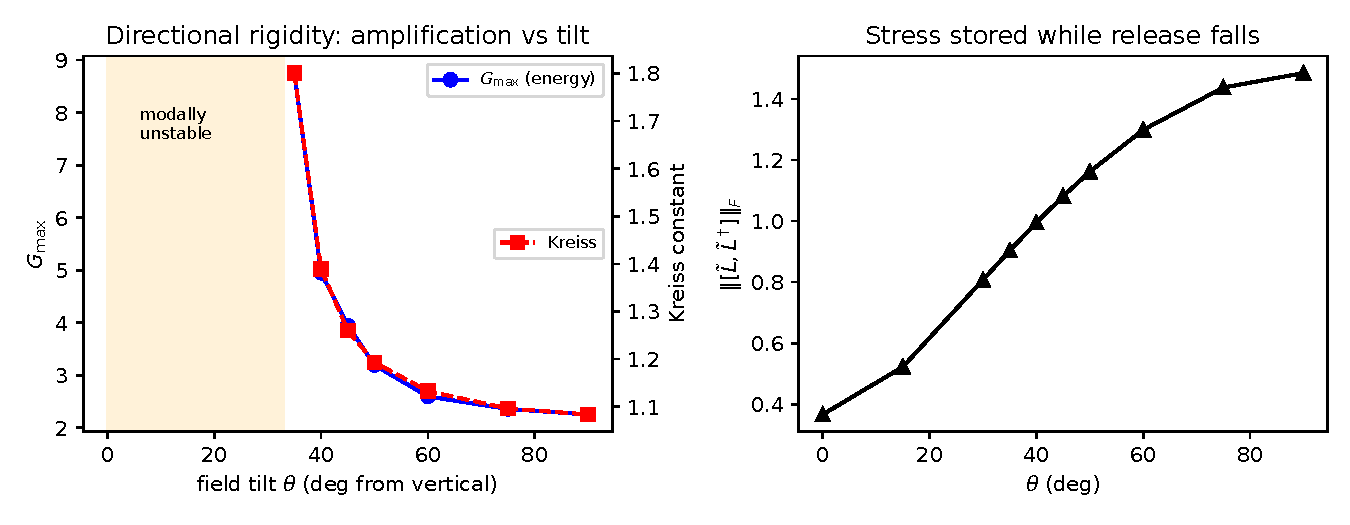
\includegraphics[width=0.95\textwidth]{figS1_lane.pdf}
\caption{SHEAR-LANE-01 (\texttt{FIG-SUNS-01}). Left: the directional-rigidity
curve---maximum transient energy growth and Kreiss constant versus field
tilt; the shaded band is the modally unstable range ending at the measured
quench. Right: the commutator stress of the same operator rises as
amplification falls: stress stored, not released.}
\label{fig:lane}
\end{figure}

\section{Comparison with the resolved vortices}\label{sec:compare}
Equation~\eqref{eq:ratio} is the only quantity the lane operator contributes
to this section, and it is fixed by the computation alone. Three comparisons
follow, in increasing order of how much they can be argued with. The script
is \texttt{DKIST-COMPARE-02} (Appendix~A.8).

\subsection{The growth rate}
Taking only the observed peak wavelength, $\lambda=65$~km,
Eq.~\eqref{eq:ratio} fixes $d=4.66$~km. The peak temporal rate for a
$\tanh$ layer is $\sigma_{\max}\approx0.19\,\Delta U/(2d)$
\cite{michalke}, and the reported apparent speeds are
$0.67$--$3.0$~km\,s$^{-1}$. This gives
\[
\sigma_{\rm pred} \;=\; 0.0137\ \mathrm{s^{-1}}\ \text{(slow end)}
\qquad\text{to}\qquad
0.0612\ \mathrm{s^{-1}}\ \text{(fast end)},
\]
against a measured $0.014$--$0.054$~s$^{-1}$: two percent at the slow end,
thirteen at the fast end. The growth rate is not an input to the prediction,
and no width convention enters the calculation [V].

What this establishes is that the photospheric layer behaves as a classical
$\tanh$ shear layer at the observed scale---the premise on which the rest of
\S\ref{sec:lane} is built, now checked rather than assumed. It is not by
itself a test of the inclination results below, which are what the framework
contributes beyond the classical picture.

\subsection{The layer width}
The observers' companion calculation gives a shear layer of approximately
$12$~km. Converting between a $\tanh$ half-width and a reported ``layer
width'' is convention-dependent; standard choices span $2d$ (the scale
width) to $4d$ ($96\%$ of the velocity jump). Their $12$~km therefore
corresponds to $d$ between $3.0$ and $6.0$~km, and by Eq.~\eqref{eq:ratio}
to a predicted wavelength between $41.9$ and $83.8$~km. The observed peak of
$65$~km lies inside that band [V]. Run in the other direction, the observed
wavelength implies $2d=9.3$~km, $2.94d=13.7$~km and $4d=18.6$~km, and their
$12$~km sits at $2.58\,d$.

The prediction of \S\ref{sec:lane}---that the true lane widths lie just below
the current resolution---therefore survives under every convention: all place
the width between $9$ and $19$~km, below the $19$~km floor. It is a
prediction the instrument cannot yet resolve, which is the point of making
it. Stating a width convention in the observational analysis would collapse
the band above to a single number and make the comparison a pass or a fail.

\subsection{The inclination curve}
This is the part not yet touched by observation. The computation gives a
critical inclination between $30^\circ$ and $35^\circ$, beyond which the mode
is quenched, and a spacing-to-width ratio that rises with tilt: $3.5$, $3.9$,
$4.5$, $6.3$ at $0^\circ$, $10^\circ$, $20^\circ$, $30^\circ$ --- the ratio is
defined only inside the modally unstable band, and by $45^\circ$ the layer is
stable with no fastest-growing mode. A follow-up
analysis of the same observation establishes that fields $1^\circ$--$7^\circ$
from exact perpendicular remain Kelvin--Helmholtz unstable \cite{nykyri},
which is consistent with the computation and approaches the quench boundary
from below without reaching it.

The decisive test is a single analysis: bin the forty-seven vortices by local
field inclination. The same observed wavelength implies lane widths of
$18.6$, $16.7$, $14.4$ and $10.3$~km at those four angles, so an
inclination-resolved width measurement separates the curves in one pass. The
observers state that the field has not been measured at these scales and name
magnetic maps as the next milestone; that measurement is the gate on this
section.

\section{The hair-rate ladder}\label{sec:ladder}
Solar activity exhibits change on three qualitatively different clocks, and
the non-normal operator family supplies exactly three rates, none of which
requires an unstable eigenvalue:
\begin{center}
\begin{tabular}{lll}
\hline
rung & operator quantity & solar face \\ \hline
slow & modal eigenvalue $\mathrm{Re}\,s$ (and cycle $2\pi/\mathrm{Im}\,s$) & activity cycle, secular decay \\
fast & transient envelope $G_{\max}$ at $t_{\rm peak}$ & shear-lane vortices, emerging structure \\
hyper-fast & numerical abscissa $\omega(L)=\lambda_{\max}\!\big(\tfrac{L+L^\dagger}{2}\big)$ & impulsive onset, flare trigger scale \\
\hline
\end{tabular}
\end{center}
Section~\ref{sec:dynamo} computes all three rungs in a single damped dynamo
operator. The family cousin on the black-hole side is exact: transient
growth and transient superradiance in modally stable regimes
\cite{besson,carballo}, where the boundary condition hides most of the hair.
The sun is the panel where all three rungs face the telescope.

\section{The dynamo operator: BH-DYNAMO-01}\label{sec:dynamo}
\subsection{Setup and predictions}
The minimal Parker $\alpha\Omega$ operator \cite{parker,charbonneau} on
colatitude $x\in[0,\pi]$:
\begin{equation}
\partial_t A = \alpha_0\cos(x)\,B + \partial_x^2 A,\qquad
\partial_t B = G\,\partial_x A + \partial_x^2 B,
\end{equation}
Dirichlet, $G=\eta=1$, $N=120$. The $\alpha$--$\Omega$ coupling is
structurally non-normal. Predictions: \textbf{(PD1)}~oscillatory onset
(dynamo waves at criticality); \textbf{(PD2)}~the ladder computed at
$0.9\,\alpha_{0c}$; \textbf{(PD3)}~the birth of the oscillatory wave branch occurs at an
exceptional point---a real eigenvalue pair colliding into a complex pair with
$\kappa\sim\delta^{-1/2}$; \textbf{(PD4)}~the shifted Dunford ledger
$\frac{1}{2\pi i}\oint\log(c+z)\Tr R(z)\,dz$ stays exact through the EP;
\textbf{(PD5)}~the Parker--Yoshimura migration rule as a control.

\subsection{Results}
\emph{PD3 passed and snapped.} The wave pair is born at
$\alpha_0^*=3.8717$, and the eigenvector condition number of the colliding
pair obeys
\[
\kappa\sqrt{\delta} \;=\; 1.842,\ 1.850,\ 1.853,\ 1.853
\qquad\text{at}\qquad \delta = 0.2,\ 0.05,\ 0.0125,\ 0.003125,
\]
the square-root defectivity law to three digits over a 64-fold range
(Fig.~\ref{fig:ep}): the birth of the oscillatory wave branch in this operator occurs at a
genuine exceptional point (distinct from the instability onset, which is
steady and lies at $\alpha_{0c}=12.696$) with EP constant $\approx1.853$.

\emph{PD4 passed exactly, with its own gate.} A contour chosen to enclose the
colliding pair alone---verified by the winding integral
$\frac{1}{2\pi i}\oint\Tr R\,dz = 2.000000$---gives a shifted trace-log
ledger equal to $\sum\log(c+\lambda_{\rm pair})$ to $9\times10^{-14}$ at the
exceptional point and beside it. (A first, sloppier contour disagreed by
exactly $\log(c+\lambda_{\rm extra})$: the instrument faithfully reported an
accidentally enclosed eigenvalue. We report this because it is the correct
way to trust a ledger.) Individual eigenvector data diverges at the EP;
phase- and contour-level data does not. This is the same survival principle
verified at the shape-manifold wall in the companion paper, now on a third
operator family.

\emph{PD2: the ladder as numbers.} At $\alpha_0=0.9\,\alpha_{0c}$, in the
energy norm $E=\int(|\partial_xA|^2+|B|^2)$: slow rung
$\max\mathrm{Re}\,s=-0.063$; fast rung $G_{\max}=3.5$ at $t=0.3$ (fifty
times faster than the modal clock); hyper rung $\omega(L)=+5.84$
(Fig.~\ref{fig:ladder}): instantaneous growth at ninety times the modal
rate in an operator whose every eigenvalue is damped. A norm lesson is
recorded honestly: an unweighted $L^2$ norm on $(A,B)$ is unit-inconsistent
and distorts every growth measure---the norm-dependence of non-normal
diagnostics emphasized in the black-hole literature \cite{gasperin} applies
verbatim to dynamo operators.

\emph{PD1 failed as predicted and stands as a model fact.} The true onset of
this minimal variant is \emph{steady}: $\alpha_{0c}=12.696$ ($D_c=394$), the
EP-born wave pair remaining damped while a steady branch crosses first.
Richer $\alpha\Omega$ models onset oscillatory \cite{charbonneau}; ours does
not, and the consequence is stated plainly: in this variant, all cyclic
physics is subcritical wave-branch phenomenology---transient by nature.

\emph{PD5 inconclusive on the full domain, with diagnosis.} The full-domain
profile $\alpha\propto\cos x$ carries an exact parity degeneracy, so the
eigensolver returns standing superpositions of the migrating pair; one shear
sign yielded a clean traveling wave (phase slope $+3.03$), the other a
standing mixture. The test requires the hemispheric domain with an
equatorial boundary condition, and is carried out in \S\ref{sec:closures}.

\subsection{SUN-N-01: the integer record at the exceptional point}
The ledger result of \S5.2 shows \emph{what} survives the exceptional point;
this gate asks whether the survivor also carries a \emph{history}. Encircle
the EP in complexified parameter space, $\alpha_0(\varphi) = \alpha_0^* +
r e^{i\varphi}$ with $r=0.15$, tracking the colliding pair by continuity.
Results: after one loop the pair \emph{exchanges} ($\lambda_1
\leftrightarrow \lambda_2$, exact to $10^{-3}$); after two loops it
restores; the discriminant winding
$\tfrac{1}{2\pi}\Delta\arg(\lambda_1-\lambda_2)^2$ evaluates to
$+1.0000$ over one loop and $+2.0000$ over two; and on a fixed contour the
eigenvalue count is constant while the shifted trace-log ledger returns
single-valued to $10^{-8}$ (Fig.~\ref{fig:braid}). The surviving spectral
object of \S5.2 therefore carries an integer record of the transport
history---a braid winding attached to the birth point of the dynamo-wave branch.

Four fences. (i) The correct invariant class here is non-Hermitian
eigenvalue \emph{braiding} \cite{huzhao,wojcik}, whose mode-exchange
signature is experimentally established for microwave-cavity EPs
\cite{dembowski} and whose local structure is the Kato square-root branch
point \cite{kato}; it is \emph{not} Atiyah--Patodi--Singer spectral flow,
which requires self-adjointness this operator does not possess. (ii) The
self-adjoint ancestor of such holonomy-indexed integer records is the
Levine--Tristram signature of knot theory \cite{levine,tristram}, whose
walls are Alexander roots; we note the ancestry without claiming the
correspondence. (iii) This is an integer record carried by an operator
family, not a statement that ``the sun remembers.'' (iv) The two verified
integers of this program---the circle's $SF=1$ and the dynamo's $W=+1$---are
distinct realizations of one concept, an integer transport record, in two
different operator categories (self-adjoint spectral flow; non-Hermitian
braiding); we do not identify them.

\begin{figure}[t]
\centering
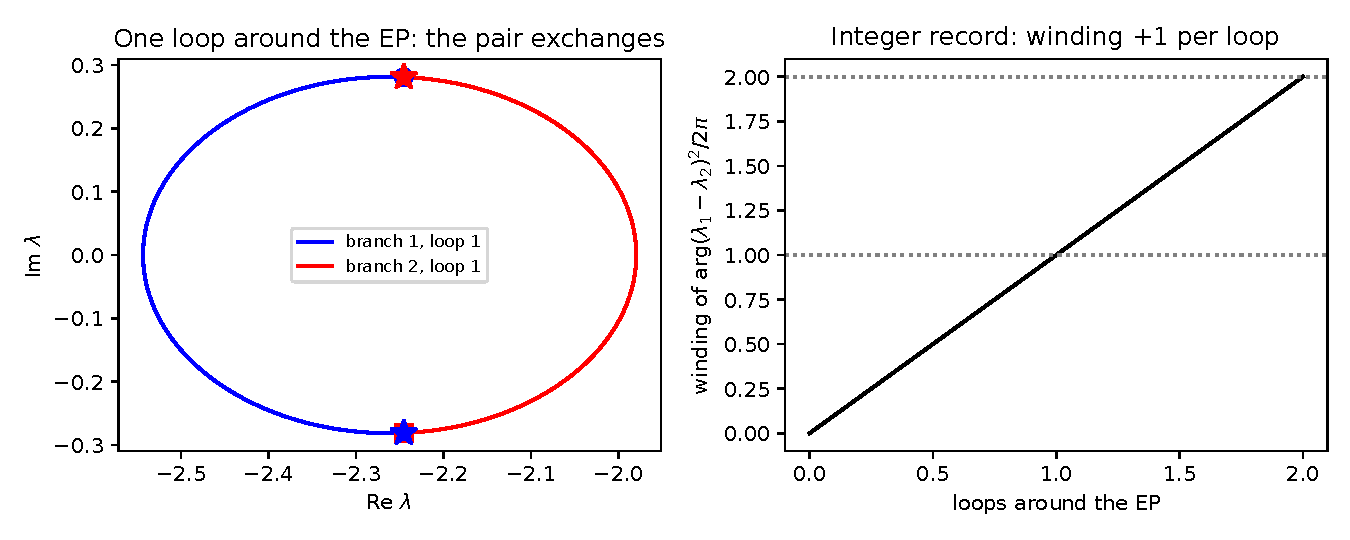
\includegraphics[width=0.95\textwidth]{figS4_braid.pdf}
\caption{SUN-N-01 (\texttt{FIG-SUNS-02}). Left: eigenvalue trajectories of
the colliding pair over one loop around the EP---each branch terminates on
the other's starting point (stars on opposite circles/squares): the exchange.
Right: the discriminant winding accumulates exactly $+1$ per loop.}
\label{fig:braid}
\end{figure}

\begin{figure}[t]
\centering
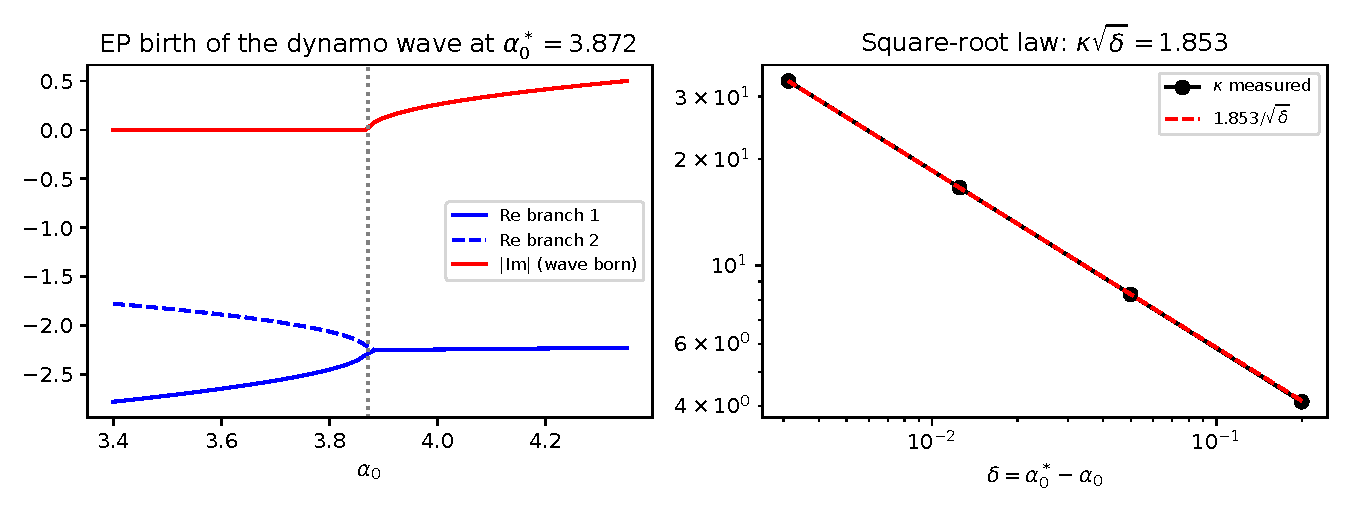
\includegraphics[width=0.95\textwidth]{figS2_ep.pdf}
\caption{BH-DYNAMO-01 (\texttt{FIG-SUNS-01}). Left: two real spectral
branches collide at $\alpha_0^*=3.872$ and a wave pair is born. Right: the
eigenvector condition number against distance from the collision, with the
square-root law $\kappa=1.853/\sqrt{\delta}$.}
\label{fig:ep}
\end{figure}

\begin{figure}[t]
\centering
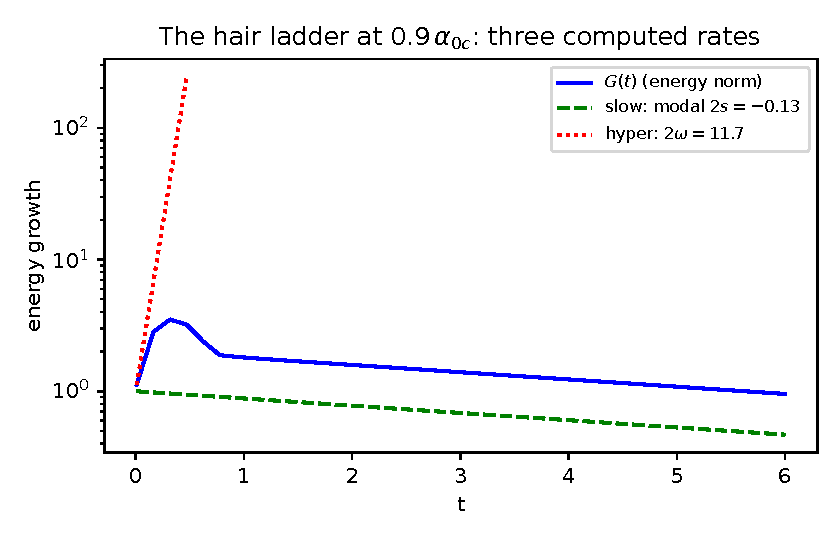
\includegraphics[width=0.55\textwidth]{figS3_ladder.pdf}
\caption{The hair-rate ladder computed in one damped operator
(\texttt{FIG-SUNS-01}): transient envelope $G(t)$ against the modal decay
line and the numerical-abscissa slope.}
\label{fig:ladder}
\end{figure}

\section{The edge census across walls}\label{sec:census}
In the companion cosmology paper, the number of projector channels trackable
from a region's boundary obeys an area law when the bulk is gapped, with a
dimensionless density: channels per correlation length of boundary,
$n_{\rm ch}\,\xi = O(1)$, measured there as exactly $1.0$ per boundary site
on a gapped lattice. The DKIST interface provides the same object at
mesoscale: discrete vortices spaced $60$--$100$~km along walls whose shear
scale is $\sim19$--$25$~km---an edge density of order $0.2$--$0.3$ per
correlation length. Reading the two together suggests a
\textbf{universality program} [H]: measure the dimensionless edge-channel
constant at every accessible rigidity interface---gapped lattices,
topological-insulator edges \cite{lihaldane}, solar shear lanes---and
determine whether it is roughly universal or strongly substrate-dependent.
The stake is stated honestly: the companion paper's horizon-channel count
extrapolates this constant to the Planck scale under a labeled gap
hypothesis; universality across accessible walls would weight that
extrapolation, while strong substrate dependence would confine it. Either
outcome is progress. The solar entry in the table should come not from the
hand inversion above but from the linearized lane operator itself
(\S\ref{sec:lane}), whose fastest-growing spacing supplies the theoretical
ratio, and from next-generation lane-width measurements. We do not claim
an observed solar measurement of $n_{\rm ch}\,\xi$; this section proposes a
cross-system diagnostic.

\section{Closing the open problems: computations and worldwide data status}\label{sec:closures}
Every open problem of the first version is revisited with either a
computation (scripts \texttt{SUN-OPEN-01/02}, Appendices~A.6--A.7) or the current worldwide data
status. Closures are graded like everything else.

\subsection*{OP1 --- the Parker--Yoshimura flip: closed [V]}
On the hemispheric domain $x\in[0,\pi/2]$ with dipole parity (pole Dirichlet;
equator $B=0$, $\partial_xA=0$) the parity degeneracy of the full domain is
lifted and the least-damped wave modes travel. Measured phase slopes:
$+1.25$ for $G=+1$ (poleward drift) and $-0.36$ for $G=-1$ (equatorward
drift): the migration direction flips with $\mathrm{sign}(\alpha G)$, and the
solar-like equatorward butterfly occurs for negative dynamo number
(Fig.~\ref{fig:butterfly}). Honest note: the two signs select different
least-damped branches, so the magnitudes are not mirror images; the tested
prediction is the sign flip, and it holds.

\begin{figure}[t]
\centering
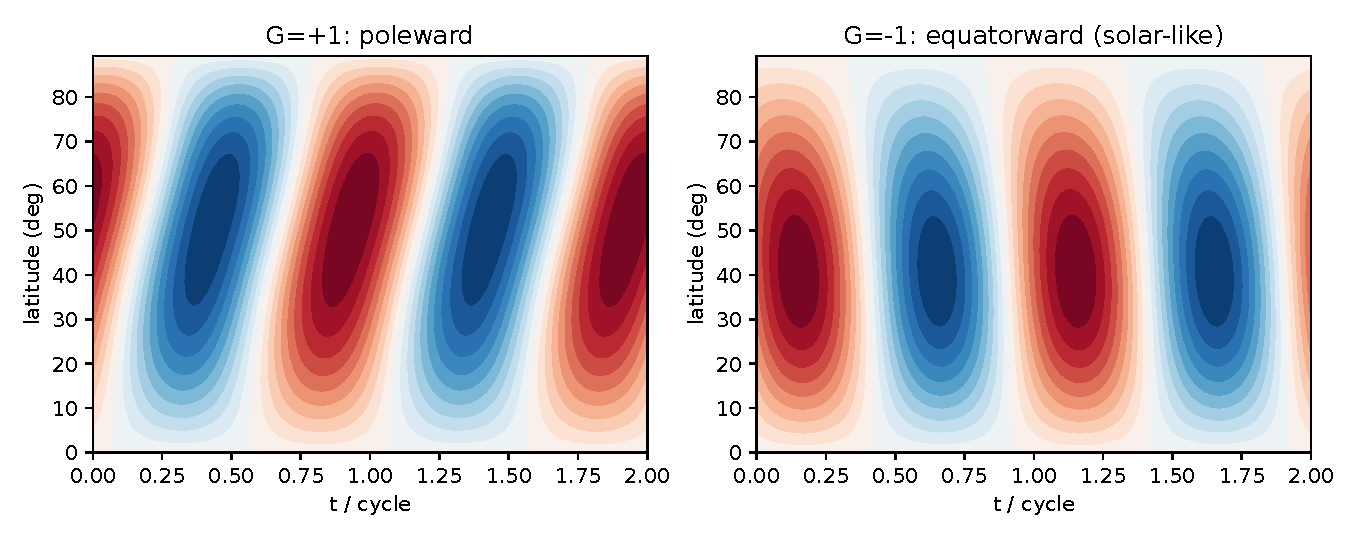
\includegraphics[width=0.95\textwidth]{figS5_butterfly.pdf}
\caption{Hemispheric butterfly diagrams from the leading wave mode
(\texttt{FIG-SUNS-03}): the migration direction flips with the sign of the
dynamo number; negative $\alpha G$ gives the solar-like equatorward drift.}
\label{fig:butterfly}
\end{figure}

\subsection*{OP2 --- oscillatory onset: mechanism closed [V]; quantitative model open}
The hemispheric dipole-parity variant also onsets steady
($\alpha_{0c}=12.53$): within the one-dimensional family the steady branch
always crosses first. The missing ingredient is now identified and verified:
a minimal two-dimensional shell ($r\in[0.2,1]\times[0,\pi]$, Dirichlet,
$\alpha\propto\cos x$ uniform in $r$) onsets \emph{oscillatory} for
\emph{either} shear orientation---the leading branch carries a growing
frequency from small drive and crosses at $s_c = 0.0000 + 49.4i$
($\alpha_{0c}\approx1665$ at $16\times32$), with the oscillatory branch
persisting at $22\times44$ (script \texttt{SUN-OPEN-02b}). Introducing radial structure provides a minimal, demonstrated route to
oscillatory onset in this operator family; the result persists under
resolution refinement and is insensitive to the tested shear orientation.
The one-dimensional steady onset is therefore not generic to the extended
family. (This demonstrates a mechanism; it is not a causal isolation of
radial structure as the unique ingredient.) The onset value is resolution- and
boundary-condition-sensitive in this deliberately crude toy, so no solar
numbers are claimed; the physically calibrated shell is merged into OP7's
remaining work, consistent with standard axisymmetric mean-field practice
\cite{charbonneau}.

\subsection*{OP3 --- the grid-optimized envelope: two-dimensional part closed [V]}
Maximizing transient growth over a discrete wavenumber--time grid
($k\in\{0.15,\ldots,0.8\}$; grid maxima are lower bounds on the true
envelope): $G_{\max}=14.8$ at $k=0.35$
($\theta=35^\circ$), $14.5$ at $k=0.15$ ($45^\circ$), $6.0$ at $k=0.15$
($60^\circ$), against fixed-$k$ values $8.8/3.8/2.5$. Two findings: the
optimal wavenumber migrates to longer waves as tilt increases (long waves
evade tension), and the grid-optimized directional-rigidity curve remains
monotone but is far flatter at small tilts than Fig.~\ref{fig:lane}---any
data comparison must use the optimized envelope. Three-dimensional
mechanisms remain cited to \cite{fraser}.

\subsection*{OP4 --- inclination-binned statistics: narrowed to one missing quantity}
The observational study is published \cite{dkist}, and three of its
distributions now bear directly on \S\ref{sec:compare}: the wavelengths
($25$--$170$~km, peaked at $65$), the apparent speeds
($0.67$--$3.0$~km\,s$^{-1}$) and the linear growth rates
($0.014$--$0.054$~s$^{-1}$). All three are consistent with the lane operator,
the growth rates quantitatively and without any fitted parameter.

What remains missing is a single quantity: the magnetic field inclination at
the vortex sites. It is exactly the variable both remaining predictions are
functions of---the quench angle and the spacing-to-width curve---and the
observers state that the field has not been measured at these scales, naming
magnetic maps as the next milestone. The protocol stands on record: bin the
forty-seven interfaces by measured inclination, compare vortex prevalence
against the optimized envelope of OP3, and compare the inclination-resolved
widths against the four values of \S\ref{sec:compare}. This is the one
genuinely external gate remaining in the paper.

\subsection*{OP5 --- the solar edge constant: theory closed [V]; observational entries [C]}
Theory: the fastest-growing spacing per lane full-width \emph{rises} with
tilt: $3.5\ (0^\circ) \to 3.9\ (10^\circ) \to 4.5\ (20^\circ) \to 6.3\
(30^\circ)$---a second falsifiable signature: spacing-to-width should
increase with field inclination. Observation: an independent DKIST/VBI
striation study \cite{striae} measures striae widths of $\approx20$--$50$~km
(below the reach of 1-m-class telescopes; simulations show $\sim100$~G
variations and Wilson depressions down to $10$~km), overlapping the
$17$--$29$~km lane widths predicted in \S\ref{sec:lane} at the lower end; and
the companion calculation of \cite{dkist} gives a shear layer of $\approx12$
~km, which \S\ref{sec:compare} places at $2.58\,d$ against the observed
wavelength. The dimensionless census entry: spacing $60$--$100$~km over width
$20$--$50$~km gives $1.2$--$5$, bracketing the $\theta=0$ prediction of
$3.5$. Equivalently, for the observed $60$--$100$~km spacings the predicted
lane full-widths are $17.1$--$28.6$~km ($0^\circ$), $15.4$--$25.6$~km
($10^\circ$), $13.3$--$22.2$~km ($20^\circ$), and $9.5$--$15.9$~km
($30^\circ$): narrower lanes under more inclined fields, at fixed spacing.

\subsection*{OP6 --- stored stress and flare statistics: sharpened; open}
Worldwide status: flare waiting-time distributions carry power-law tails
$\Delta t^{-\alpha}$ with $\alpha\approx1.5$--$3.2$ across instruments and
$2$--$3$ per cycle \cite{aschrev,biasiotti}; hard X-ray catalogs give mean
waiting $0.80$~h with tail slope $\approx2.0$; the classical account is a
nonstationary Poisson process whose measured rate distribution
$f(\lambda)\sim\lambda^{-0.9}$ reproduces the $-2.2$ tail \cite{wheatland};
the 2026 far-side-inclusive analysis finds the extreme active region
log-normal and the global tail steeper than $3$, defying the local Poisson
hypothesis \cite{wtd2026}; a CNN catalog of $111{,}580$ events steepens the
size index to $-2.59$ \cite{cnncat}. The framework's qualitative
prediction---release gated by slowly accumulated stored stress, hence
strongly non-Poisson occurrence---is what is observed, but observation does
not single out the mechanism. The sharpened target: derive the rate
distribution $f(\lambda)$ from a $\Phi$-storage reservoir fed by the lane
operator's stress budget and released at the hyper-fast rung, and compare
with the measured $\lambda^{-0.9}$.

\emph{A measured reservoir.} The follow-up analysis of the same observation
supplies the missing scale: a shear-energy density of
$1.35\times10^{2}$~J\,m$^{-3}$ and $2.2\times10^{24}$~erg per characteristic
vortex over a $500$~km vertical extent \cite{nykyri}. The stored-versus-
released distinction of \S\ref{sec:lane}---$\Phi$ rising with tilt while
realizable growth falls---is a statement about the ratio of those two
quantities as a function of inclination, and a published reservoir per vortex
makes that ratio a measurable rather than a schematic object. It is the
natural input to the hazard programme below.

\emph{Statistical-inverse closure [V under a stated ansatz].} The
nonstationary-Poisson relation gives the waiting-time tail exponent $3+\beta$
for a rate distribution $f(\lambda)\sim\lambda^{\beta}$; the measured
$\beta=-0.9$ reproduces the observed $\approx2.1$ tail \cite{wheatland}.
Inverting the reservoir picture---constant charging $\dot\Phi\approx q$, a
monotone hazard $\lambda(\Phi)$, renewal on release---the time-spent measure
$f(\lambda)\propto d\Phi/d\lambda$ forces $\Phi\propto\lambda^{1+\beta}$,
i.e.
\[
\lambda \;\propto\; \Phi^{1/(1+\beta)} \;=\; \Phi^{10}
\quad (\beta=-0.9).
\]
The exponent is razor-sensitive to $\beta$'s error bar ($\beta=-0.8$ gives
$\Phi^{5}$; $\beta\to-1$ gives a logarithmic hazard), so the robust
statement is: \emph{the reservoir hazard is steeper than $\Phi^{5}$}---a stiff gate: at exponent $10$ a $7.2\%$ stress rise doubles the rate
($2^{1/10}=1.072$), and a $26\%$ rise increases it roughly tenfold
($1.26^{10}\approx10$).
Two honest cautions: the ansatz (constant charging, monotone hazard,
renewal) is named, not derived; and the tilt-scan $\Phi$ range of
\S\ref{sec:lane} is a control-parameter scan, not temporal charging, so it
illustrates the operator's stress range only. Status: closed at the
statistical-inverse level; the first-principles hazard remains open.

\subsection*{OP7 --- spherical models: first step taken}
The hemispheric computation is the first step off the full-line toy, and the
ledger and EP machinery run on it unchanged. Spherical $(r,\theta)$
mean-field models and contact with the optimal-dynamo program
\cite{chenlivermore,herreman} remain open. The shell computation under OP2
demonstrates the mechanism this calibration will inherit.

\subsection*{OP8 --- the braid census: closed [V], with a structural resolution}
Scanning $\alpha_0\in(0,13]$: the exceptional set is a \emph{ladder} of
pair-birth points at $\alpha_0^* = 3.872$, $5.280$, $7.158$, $9.085$
and $11.032$.
Encircling every one of the five with radial-continuation tracking (select
the newborn conjugate pair just above each birth point, continue it out to
the loop radius, then around) gives winding $+1.0000$ with pair exchange resolved to tolerance
$5\times10^{-3}$ at \emph{all five resolved} points in $0<\alpha_0\le13$
(script \texttt{SUN-OPEN-02}). And the ``real two-parameter loop'' question resolves structurally:
for real operator families, real-to-complex collisions occur on
codimension-one sets---walls, not points \cite{kato}---so encirclement
intrinsically requires complexification. The braid record is a property of
the complexified family, read on the real axis as wall crossings.

\section{Remaining open problems}
\begin{enumerate}
\item Field inclination at the vortex sites---the one genuinely external
gate. When magnetic maps at vortex scale exist, the binning of
\S\ref{sec:compare} tests the quench angle and the spacing-to-width curve in
a single analysis.
\item The first-principles hazard: derive $\lambda(\Phi)$ and $f(\lambda)$
from the stress reservoir rather than inverting them, now with a measured
reservoir per vortex as input (OP6).
\item The physically calibrated shell/spherical solar model, inheriting the
verified oscillatory-onset mechanism (OP2+OP7).
\item A stated width convention in the observational analysis, which would
collapse the band of \S\ref{sec:compare} to a single number.
\end{enumerate}

\appendix
\section{Scripts}
Every number in this paper is generated by the scripts below, listed in full.
Each carries its name in a header comment; dependencies are \texttt{numpy},
\texttt{scipy}, \texttt{matplotlib}.

\subsection*{A.1 \ SHEAR-LANE-01}
\lstinputlisting{shear_lane_01.py}
\subsection*{A.2 \ BH-DYNAMO-01}
\lstinputlisting{bh_dynamo_01.py}
\subsection*{A.3 \ BH-DYNAMO-01b (fix pass)}
\lstinputlisting{bh_dynamo_01b.py}
\subsection*{A.4 \ FIG-SUNS-01 (figures 1--3)}
\lstinputlisting{fig_suns_01.py}
\subsection*{A.5 \ N-RECOVERY-01b (the SUN-N-01 loop) and FIG-SUNS-02}
\lstinputlisting{n_recovery_01b.py}
\lstinputlisting{fig_suns_02.py}
\subsection*{A.6 \ SUN-OPEN-01 (closures) and FIG-SUNS-03}
\lstinputlisting{sun_open_01.py}
\lstinputlisting{fig_suns_03.py}
\subsection*{A.7 \ SUN-OPEN-02 and SUN-OPEN-02b (full census, shell onset)}
\lstinputlisting{sun_open_02.py}
\lstinputlisting{sun_open_02b.py}
\subsection*{A.8 \ DKIST-COMPARE-02 (the comparison of \S\ref{sec:compare})}
\lstinputlisting{dkist_compare_02.py}

\section*{Acknowledgments}
Computational verification, gating, and drafting assistance by an AI
collaborator (Claude, Anthropic); every gate above is independently
re-runnable from Appendix~A. License: CC BY 4.0.

\begin{thebibliography}{99}
\bibitem{dkist} D.~Kuridze et al., Ubiquitous Kelvin--Helmholtz
instabilities driving plasma mixing on the Sun, Nature (2026),
doi:10.1038/s41586-026-10871-3; MPS/NSF--NSO press release 26900660.
\bibitem{nykyri} K.~Nykyri, Photospheric Kelvin--Helmholtz vortices as
possible drivers of coronal heating: implications of the DKIST observations,
arXiv:2608.12796 (2026).
\bibitem{striae} The striated solar photosphere observed at $0.03''$
resolution, Astrophys.\ J.\ Lett.\ (2025); arXiv:2505.03965.
\bibitem{aschrev} M.~J.~Aschwanden and T.~Dudok de Wit, Waiting-time
distributions of solar flares, coronal mass ejections, and radio bursts,
Astrophys.\ J.\ (2021).
\bibitem{wheatland} M.~S.~Wheatland, Understanding solar flare waiting-time
distributions, Solar Phys.\ (2003).
\bibitem{biasiotti} L.~Biasiotti and S.~L.~Ivanovski, Statistical analysis
of solar flare properties from 1975 to 2017, Solar Phys.\ \textbf{300}, 121
(2025).
\bibitem{wtd2026} Waiting time distribution of solar flares from a global
perspective, Astrophys.\ J.\ Lett.\ (2026); arXiv:2604.00877.
\bibitem{cnncat} A convolutional neural network--derived catalog of solar
flares from soft X-ray observations, Astrophys.\ J.\ Suppl.\ (2026).
\bibitem{rimmele} T.~R.~Rimmele et al., The Daniel K. Inouye Solar
Telescope: Observatory overview, Solar Phys.\ \textbf{295}, 172 (2020).
\bibitem{fraser} A.~E.~Fraser et al., Nonmodal growth and optimal
perturbations in magnetohydrodynamic shear flows, Phys.\ Rev.\ E (2026);
arXiv:2510.03141.
\bibitem{michalke} A.~Michalke, On the inviscid instability of the
hyperbolic-tangent velocity profile, J.\ Fluid Mech.\ \textbf{19}, 543
(1964).
\bibitem{chandra} S.~Chandrasekhar, \emph{Hydrodynamic and Hydromagnetic
Stability}, Oxford (1961).
\bibitem{keppens} R.~Keppens, G.~T\'oth, R.~H.~J.~Westermann, and
J.~P.~Goedbloed, Growth and saturation of the Kelvin--Helmholtz instability
with parallel and anti-parallel magnetic fields, J.\ Plasma Phys.\
\textbf{61}, 1 (1999).
\bibitem{obergaulinger} M.~Obergaulinger et al., Local simulations of the
magnetized Kelvin--Helmholtz instability in neutron-star mergers, Astron.\
Astrophys.\ \textbf{515}, A30 (2010).
\bibitem{mactaggart} D.~MacTaggart, Optimal energy growth in current
sheets, Solar Phys.\ \textbf{293}, 148 (2018).
\bibitem{trefethen93} L.~N.~Trefethen, A.~E.~Trefethen, S.~C.~Reddy, and
T.~A.~Driscoll, Hydrodynamic stability without eigenvalues, Science
\textbf{261}, 578 (1993).
\bibitem{trefembree} L.~N.~Trefethen and M.~Embree, \emph{Spectra and
Pseudospectra}, Princeton (2005).
\bibitem{farrell} B.~F.~Farrell and P.~J.~Ioannou, Generalized stability
theory. Part I, J.\ Atmos.\ Sci.\ \textbf{53}, 2025 (1996).
\bibitem{parker} E.~N.~Parker, Hydromagnetic dynamo models, Astrophys.\ J.\
\textbf{122}, 293 (1955).
\bibitem{yoshimura} H.~Yoshimura, Solar-cycle dynamo wave propagation,
Astrophys.\ J.\ \textbf{201}, 740 (1975).
\bibitem{charbonneau} P.~Charbonneau, Dynamo models of the solar cycle,
Living Rev.\ Sol.\ Phys.\ \textbf{17}, 4 (2020).
\bibitem{chenlivermore} L.~Chen, W.~Herreman, K.~Li, P.~W.~Livermore,
J.~W.~Luo, and A.~Jackson, Optimal kinematic dynamos in a sphere, Proc.\
R.\ Soc.\ A \textbf{476}, 20190675 (2020).
\bibitem{herreman} W.~Herreman, Minimal perturbation flows that trigger
mean field dynamos in shear flows, J.\ Plasma Phys.\ \textbf{84},
735840305 (2018).
\bibitem{kirillov} O.~N.~Kirillov, \emph{Nonconservative Stability Problems
of Modern Physics}, De Gruyter (2013).
\bibitem{jaramillo} J.~L.~Jaramillo, R.~Panosso Macedo, and L.~Al Sheikh,
Pseudospectrum and black hole quasinormal mode instability, Phys.\ Rev.\ X
\textbf{11}, 031003 (2021).
\bibitem{gasperin} E.~Gasperin and J.~L.~Jaramillo, Energy scales and black
hole pseudospectra: the structural role of the scalar product, Class.\
Quantum Grav.\ \textbf{39}, 115010 (2022).
\bibitem{besson} J.~Besson, J.~Carballo, C.~Pantelidou, and B.~Withers,
Transients in black hole perturbation theory, Front.\ Phys.\ \textbf{13},
1638583 (2025).
\bibitem{carballo} J.~Carballo, C.~Pantelidou, and B.~Withers, Transient
superradiance, JHEP \textbf{08}, 179 (2025).
\bibitem{lihaldane} H.~Li and F.~D.~M.~Haldane, Entanglement spectrum as a
generalization of entanglement entropy, Phys.\ Rev.\ Lett.\ \textbf{101},
010504 (2008).
\bibitem{huzhao} H.~Hu and E.~Zhao, Knots and non-Hermitian Bloch bands,
Phys.\ Rev.\ Lett.\ \textbf{126}, 010401 (2021).
\bibitem{wojcik} C.~C.~Wojcik, X.-Q.~Sun, T.~Bzdu\v{s}ek, and S.~Fan,
Homotopy characterization of non-Hermitian Hamiltonians, Phys.\ Rev.\ B
\textbf{101}, 205417 (2020).
\bibitem{dembowski} C.~Dembowski et al., Experimental observation of the
topological structure of exceptional points, Phys.\ Rev.\ Lett.\
\textbf{86}, 787 (2001).
\bibitem{kato} T.~Kato, \emph{Perturbation Theory for Linear Operators},
Springer (1966).
\bibitem{levine} J.~Levine, Knot cobordism groups in codimension two,
Comment.\ Math.\ Helv.\ \textbf{44}, 229 (1969).
\bibitem{tristram} A.~G.~Tristram, Some cobordism invariants for links,
Proc.\ Camb.\ Phil.\ Soc.\ \textbf{66}, 251 (1969).
\bibitem{foft} J.~N.~Beasley, Foundational Operator Field Theory on
Stratified Manifolds, v2 (2026), companion paper.
\bibitem{blkhole} J.~N.~Beasley, Beyond the Event Horizon: Operator
Decoupling at the Rigidity Wall, v2 (2026), companion paper.
\end{thebibliography}

\end{document}
